\subsection{ALGEBRA OF A MAGMA, A MONOID, A GROUP}

Recall that a magma is a set with a law of composition (I, § 1, no. 1). Let S be a magma written multiplicatively and let \(\mathbf{E} = \mathbf{A}^{(\mathbb{S})}\) be the A-module of formal linear combinations of elements of S (II, § 1, no. 11); we know that a canonical mapping \(s \mapsto e_s\) is defined of S into \(\mathbf{A}^{(\mathbb{S})}\) such that the family \((e_s)_{s \in \mathbb{S}}\) is a basis (called canonical) of \(\mathbf{A}^{(\mathbb{S})}\) , every element of \(\mathbf{A}^{(\mathbb{S})}\) being then written uniquely in the form \(\sum_{s \in \mathbb{S}} \alpha_s e_s\) , where \((\alpha_s)\) is a family of elements of A of finite support. Then an A-algebra structure is defined on E by taking as multiplication table of the canonical basis

\[
e _ {s} e _ {t} = e _ {s t}\tag{35}
\]

The algebra E thus defined is called the algebra of the magma S over A. If \(x = \sum_{s \in S} \xi_{s} e_{s}\) and \(y = \sum_{s \in S} \eta_{s} e_{s}\) are two elements of E, then

\[
x y = \sum_ {s \in \mathbb {S}} \left(\sum_ {t u = s} \xi_ {t} \eta_ {u}\right) e _ {s}.
\]

When S is a monoid (resp. group), E is called the algebra of the monoid (resp. group) S over A; it is then an associative algebra (§ 1, no. 7); similarly, when S is a commutative monoid, its algebra is associative and commutative. Finally if the magma S admits an identity element \(u\) , \(e_u\) is unit element of the algebra E; as the element \(e_u\) is free, A is then identified with the subalgebra \(Ae_u\) of E.

When \(A \neq \{0\}\) , S is sometimes identified with its image under the injection \(s \mapsto e_{s}\) , so that an element of E is written as \(\sum_{s \in S} \alpha_{s}s\) ; but this identification is not possible (without causing confusion) when S is written additively. Then \(e^{s}\) is also often written instead of \(e_{s}\) .

Let B be another commutative ring and \(\rho: A \to B\) a ring homomorphism; consider the algebras \(E = A^{(S)}\) and \(E' = B^{(S)}\) of the same magma S over A and B and let \((e_s)_{s \in S}\) and \((e_s')_{s \in S}\) be their respective canonical bases. The algebra \(B^{(S)}\) is canonically identified, under the A-linear mapping \(j\) such that \(j(e_s \otimes 1) = e_s'\) for all \(s \in S\) , with the algebra \(A^{(S)} \otimes_A B\) obtained from \(A^{(S)}\) by extending the ring of scalars to B (II, § 1, no. 11, Corollary 3 to Proposition 17).

PROPOSITION 6. Let S be a magma, F an A-algebra and f a homomorphism of

S into F with only its multiplicative structure. Then there exists one and only one A-algebra homomorphism \(\bar{f}:\mathbf{A}^{(\mathbb{S})}\to\mathbf{F}\) rendering commutative the diagram

\begin{enumerate}
\def\labelenumi{(\arabic{enumi})}
\setcounter{enumi}{35}
\tightlist
\item
\end{enumerate}

\pandocbounded{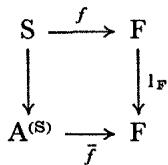
\includegraphics[keepaspectratio]{images/part003_a94682a2.jpg}}

(where the vertical arrow on the left is the canonical mapping \(s \mapsto e_s\) ).

Let \(\bar{f}:\mathbf{A}^{(\mathrm{S})}\to\mathbf{F}\) be the unique A-module homomorphism such that \(\bar{f}(e_{s})=\bar{f}(s)\) (II, §1, no. 11, Corollary 3 to Proposition 17); it suffices to verify that \(\bar{f}\) is an algebra homomorphism and for this it suffices to prove that \(\bar{f}(e_{s}e_{t})=\bar{f}(e_{s})\bar{f}(e_{t})\) , which follows immediately from the definition and the hypothesis \(f(st)=f(s)f(t)\) .

Proposition 6 expresses the fact that the ordered pair consisting of \(\mathbf{A}^{(\mathbb{S})}\) and the canonical mapping \(s\mapsto e_s\) is a solution of the universal mapping problem (Set Theory, IV, §3, no. 1) where \(\Sigma\) is the species of A-algebra structure and the \(\alpha\) -mappings the homomorphisms of S into an A-algebra with only its multiplicative law.

COROLLARY. Let S, S' be two magmas and \(g:S\to S'\) a homomorphism. Then there exists one and only one A-algebra homomorphism \(u:A^{(S)}\to A^{(S')}\) rendering commutative the diagram

\pandocbounded{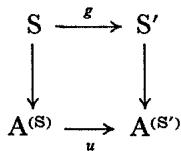
\includegraphics[keepaspectratio]{images/part003_71823134.jpg}}

(where the vertical arrows are the canonical mappings).

It suffices to apply Proposition 6 taking \(f\) to be the composite mapping \(\mathbf{S} \xrightarrow{g} \mathbf{S}' \to \mathbf{A}^{(\mathbf{S}')}\) .

In particular, if T is a stable subset of the magma S (I, § 1, no. 4), the set of elements \(\sum_{s\in\mathbf{T}}\alpha_s e_s\) of \(\mathbf{A}^{(\mathbf{S})}\) is a subalgebra of \(\mathbf{A}^{(\mathbf{S})}\) canonically isomorphic to the algebra \(\mathbf{A}^{(\mathbf{T})}\) and sometimes identified with the latter.

Example. Let V be an A-module and S a monoid which operates on V on the left; this means (I, § 5, no. 1) that there is given a mapping \((s, x) \mapsto s.x\) of S into V such that \(s.(x + y) = s.x + s.y\) , \(s.(\alpha x) = \alpha(s.x)\) and \(s.(t.x) = (st).x\) for \(s, t\) in S, \(x, y\) in V and \(\alpha \in \mathbf{A}\) and, denoting by \(e\) the identity element of S, e.x = x for \(x \in V\) . Writing \(f(s)(x) = s.x\) , f is a homomorphism of S into the algebra \(\operatorname{End}_{\mathbf{A}}(\mathbf{V})\) (with only its multiplicative law), mapping the identity element e to the unit element \(1_{V}\) . Applying Proposition 6, an A-algebra homomorphism \(\bar{f}: \mathbf{A}^{(\mathbf{S})} \to \operatorname{End}_{\mathbf{A}}(\mathbf{V})\) is obtained, which gives the underlying group of V a left module structure over \(\mathbf{A}^{(\mathbf{S})}\) .

This allows us to reduce the study of commutative groups with operators to that of modules. For let M be a commutative group with operators written additively, all of whose external laws are written multiplicatively. Let \(\Omega\) be the sum set (Set Theory, II, §4, no. 8) of the domains of operators of the various external laws on M, each of these domains being canonically identified with a subset of \(\Omega\) . Let \(\mathrm{Mo}(\Omega)\) be the free monoid (I §7, no. 2) constructed on \(\Omega\) ; a law of action

\[
(s, x) \mapsto s. x
\]

is defined on M with \(\mathrm{Mo}(\Omega)\) as domain of operators, by induction on the length of the word s in \(\mathrm{Mo}(\Omega)\) ; if s is of length 0, it is the empty word e and we write e.x = x for all \(x \in M\) . If x is of length \(n \geqslant 1\) , it can be written uniquely as s = tu, where u is of length n - 1 and t of length 1, so that \(t \in \Omega\) ; we then write s.x = t.(u.x). For any two words s, \(s'\) in \(\mathrm{Mo}(\Omega)\) , the relation \(s.(s'.x) = (ss').x\) is verified by induction on the length of s.

Then applying the method described above, a left \(\mathbf{Z}^{(\mathrm{Mo}(\Omega))}\) -module structure is obtained on M and it is verified without difficulty that the usual notions in the theory of groups with operators (stable subgroups, homomorphisms) are the same for commutative groups with operators and the modules thus associated with them.

